% !TeX root=main.tex

\section{Methodik der Thesis}

Die Methodik dieser Bachelorarbeit basiert auf einer Kombination aus Literaturrecherche, Fallstudienanalyse und empirischen Untersuchungen. Diese Methodenkombination ermöglicht es, ein fundiertes theoretisches Fundament zu legen und gleichzeitig praktische Einblicke und Daten zu gewinnen, um die Forschungsfragen zu beantworten.

\begin{figure}[H]
    \centering
    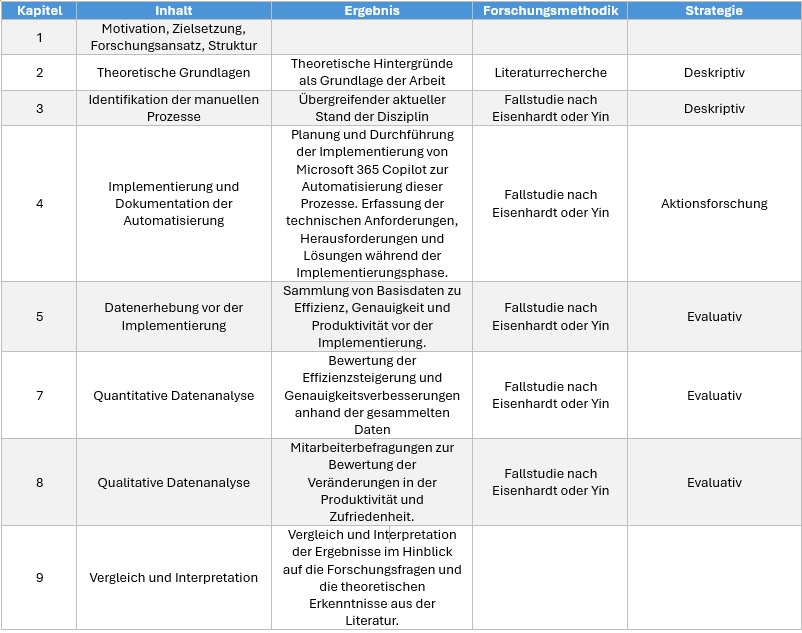
\includegraphics[scale=0.6]{methodik}
    \captionsetup{font=scriptsize}
    \caption{Aufbau und Struktur der Bachelorthesis mit Forschungsmethodik}
    \label{fig:methodik}
\end{figure}

Die Methodik der Fallstudienforschung basiert auf bewährten Ansätzen, wie sie von Yin\footnote{Vgl. \cite{Yin2017}} und Eisenhardt\footnote{Vgl. \cite{Eisenhardt1989}} beschrieben wurden. Yin bietet einen umfassenden Leitfaden zur Durchführung von Fallstudien, einschließlich der Fallauswahl, Datenerhebung und Datenanalyse. Eisenhardt ergänzt diesen Ansatz durch ihre Methoden zur Theorieentwicklung aus Fallstudien. Der in dieser Arbeit verwendete Ablauf orientiert sich an diesen etablierten Methoden.

Die Methodik der Literaturrecherche basiert auf dem Ansatz von Aveyard\footnote{Vgl. \cite{Aveyard2018}} und wurde bereits begonnen.


\clearpage